\documentclass{beamer}
\usepackage[utf8]{inputenc}
\usepackage{biblatex}
\addbibresource{cite.bib}
\usetheme{CambridgeUS}
\usecolortheme{default}


\newcommand{\R}{\mathbb{R}}

\newcommand\Tstrut{\rule{0pt}{2.6ex}}

\AtBeginBibliography{\tiny}

\title[Efficient Attention]
{Efficient Attention}
\subtitle{
    And the Chronicles of LoRA the Transformer
}
\author[Chaudhary, Pawagi, Jorige, Nagasai]
{
    Sahil Chaudhary$^*$ \and Mrigank Pawagi$^*$ \\ Rohit Jorige$^*$ \and Nagasai Jajapuram$^*$ \bigskip \\
    \texttt{WorthYourAttention}
    \\
    {\tiny $^*$Equal contribution.}
}
\institute[]
{Indian Institute of Science}
\date[12 April 2024]
{12 April 2024}
\logo{}
\begin{document}

\frame{\titlepage}

\begin{frame}
    \frametitle{Introduction}
    A long long time ago... RNN's and LSTM's were the go-to model for sequence to sequence models. But they had a few flaws:
    \begin{itemize}
        \item Sequential Processing
        \item They do not accurately capture long term dependencies (not LSTM)
        \item They were slow
        \item Hard to parallelize 
        \item Past information retained through past hidden states
        \item Vanishing gradients
    \end{itemize}
    \end{frame}

    \begin{frame}
        \frametitle{Attention in Transformers}
        \framesubtitle{Overview of the architecture}
        
        % Splitting the frame into two halves
        \begin{columns}[T]
            \column{.5\textwidth}
            \textbf{Key Innovations in Transformers:}
            \begin{itemize}
                \item \textbf{Non-sequential Processing:} Sentences are processed as a whole, not word by word.
                \item \textbf{Self Attention:} A new $'$unit$'$ for computing word similarity scores within a sentence.
                \item \textbf{Positional Embeddings:} Replaces recurrence with fixed or learned weights encoding token position information.
            \end{itemize}
            \column{.5\textwidth}
            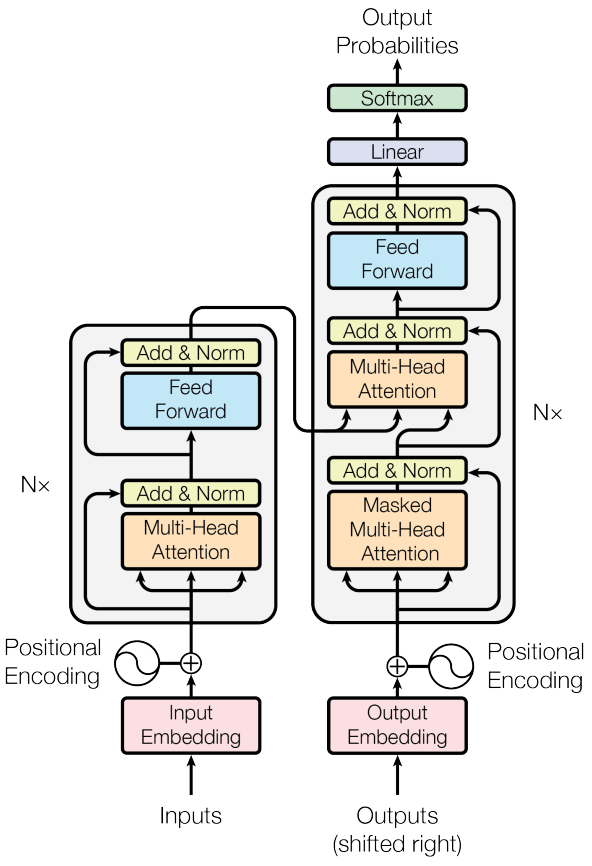
\includegraphics[width=0.8\textwidth]{images/attention_architecture.png}
        \end{columns}
    \end{frame}
    

    \begin{frame}
        \frametitle{Attention in Transformers}
        \framesubtitle{Attention Mechanism}
    
        % Splitting the frame into two halves with reduced width for images
        \begin{columns}[T]
            \begin{column}{0.4\textwidth}
                \textbf{Scaled Dot-Product Attention}\\
                \centering
                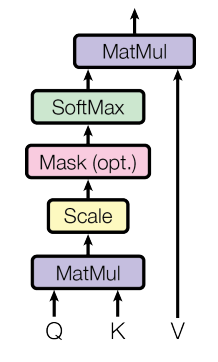
\includegraphics[width=0.4\textwidth]{images/scaled_attention.png}
                \vspace{0.5cm}
                \begin{center}
                    \begin{minipage}{\linewidth} % Create a minipage for the box
                        \tiny % Make the font size smaller
                        \boxed{\text{Attention}(Q, K, V) = \text{softmax}\left(\frac{QK^T}{\sqrt{D}}\right) V}
                    \end{minipage}
                \end{center}
            \end{column}
            \begin{column}{.4\textwidth}
                \centering
                \textbf{Multi-Head Attention}\\
                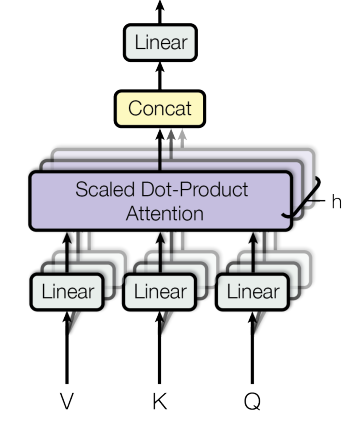
\includegraphics[width=0.6\textwidth]{images/multihead_attention.png}
                \vspace{0.5cm}
                \begin{center}
                    \begin{minipage}{\linewidth} % Create a minipage for the box
                        \tiny % Make the font size tiny
                        \boxed{\text{MultiHead}(Q, K, V) = \text{Concat}(Head_1, ..., Head_h) W_O}
                    \end{minipage}
                \end{center}
            \end{column}
        \end{columns}
    \end{frame}
    \begin{frame}
        \frametitle{English to Kannada Translation}
        \begin{center}
            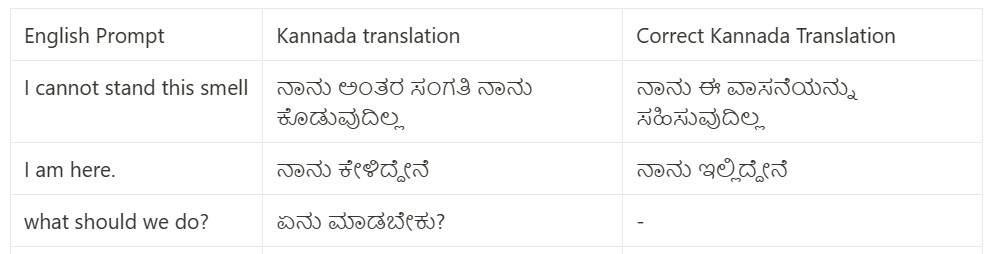
\includegraphics[width=1\textwidth]{images/kannada.png} % Adjust the width as needed
        \end{center}
    \end{frame}
    \begin{frame}
        \frametitle{Transformer Formal Definition}
        Let $x \in \mathbb{R}^{N \times F}$ denote a sequence of $N$ feature vectors of dimensions $F$.\\
        A transformer is a function $T : \mathbb{R}^{N \times F} \rightarrow \mathbb{R}^{N \times F}$ defined by the composition of $L$ transformer layers $T_1(\cdot), \ldots, T_L(\cdot)$, where
        \begin{align*}
            T_i(x) = f_i(A_i(x) + x)
        \end{align*}
        Here $f_i(\cdot)$ is usually implemented using a feed-forward network, $A_i$ is a self-attention function. 
    \end{frame}
    \begin{frame}
        \frametitle{Formal Definition}
        Formally, the input sequence $x$ is projected by three matrices $W_Q \in \mathbb{R}^{F \times D}$, $W_K \in \mathbb{R}^{F \times D}$ and $W_V \in \mathbb{R}^{F \times F}$ to corresponding representations $Q$, $K$ and $V$. The output for all positions, $A_i(x) = V'$, is computed as follows,
        \begin{align*}
            Q &= xW_Q, \\
            K &= xW_K, \\
            V &= xW_V,
        \end{align*}
        The output $A_i(x)$ is computed as follows:
    \[A_i(x) = V' = \text{softmax}\left(\frac{QK^T}{\sqrt{D}}\right)V.\]
    \end{frame} 
    \begin{frame}
    \frametitle{Linear Attention}
    \framesubtitle{Similarity Function}
    Attention on a closer look is nothing but a weighted average of the values, where the weight assigned to each value is computed by similarity function of the corresponding key.
    
    \begin{align*}
        A_i(x)=V'=\begin{bmatrix}
             \frac{\sum_{j=1}^{N}sim(Q_k,K_j)V_j}{\sum_{j=1}^{N}sim(Q_k,K_j)}
        \end{bmatrix}_{k=1}^{N}
    \end{align*}

    
    \end{frame}

    \begin{frame}{Linear Attention}
    \framesubtitle{Similarity Function}
        What are the properties we wish to have on similarity function?
        \begin{enumerate}
            \item sim:$\R^D \times \R^D \rightarrow \R_{+}$ % \pause
            % \item $sim(x,y)=sim(y,x)$ $\forall x,y \in R^D$
        \end{enumerate}
        \pause
        Note that this includes all kernels $K(x,y):\R^D \times \R^D \rightarrow \R_{+}$
    \end{frame}
    \begin{frame}{Linear Attention}
    \framesubtitle{Introduce Kernels}
    Thus, attention can be written as,
    \begin{align}
        V'=\begin{bmatrix}
        \frac{\sum_{j=1}^{N}K(Q_k,K_j)V_j}{\sum_{j=1}^{N}K(Q_k,K_j)}    
        \end{bmatrix}
    \end{align}
    \end{frame}
    \begin{frame}{Linear Attention}
    \framesubtitle{Introduce Kernels}
    Thus, attention can be written as,
    \begin{align*}
        V'=\begin{bmatrix}
        \frac{\sum_{j=1}^{N}K(Q_k,K_j)V_j}{\sum_{j=1}^{N}K(Q_k,K_j)}    
        \end{bmatrix}
    \end{align*}
    Let's look at each row of this matrix.
    \begin{align*}
        V'_k=\frac{\sum_{j=1}^{N}K(Q_k,K_j)V_j}{\sum_{j=1}^{N}K(Q_k,K_j)} 
    \end{align*}
    \end{frame}
    \begin{frame}{Linear Attention}
    Given a kernel with a feature representation $\phi(x)$, we can rewrite this as
    \begin{align*}
        V'_k=\frac{\sum_{j=1}^{N}\phi(Q_k)^T\phi(K_j)V_j}{\sum_{j=1}^{N}\phi(Q_k)^T\phi(K_j)} 
    \end{align*}
        
    \end{frame}
    \begin{frame}{Linear Attention}
    Given a kernel with a feature representation $\phi(x)$, we can rewrite $eq^n-3$ as follows,
    \begin{align*}
        V'_k&=\frac{\sum_{j=1}^{N}\phi(Q_k)^T\phi(K_j)V_j}{\sum_{j=1}^{N}\phi(Q_k)^T\phi(K_j)} \\
        V'_k&=\frac{\phi(Q_k)^T\sum_{j=1}^{N}\phi(K_j)V_j^T}{\phi(Q_k)^T\sum_{j=1}^{N}\phi(K_j)}
    \end{align*}
        
    \end{frame}
    \begin{frame}{Linear Attention}
    Given a kernel with a feature representation $\phi(x)$, we can rewrite $eq^n-3$ as follows,
    \begin{align*}
        V'_k&=\frac{\sum_{j=1}^{N}\phi(Q_k)^T\phi(K_j)V_j}{\sum_{j=1}^{N}\phi(Q_k)^T\phi(K_j)} \\
        V'_k&=\frac{\phi(Q_k)^T\sum_{j=1}^{N}\phi(K_j)V_j^T}{\phi(Q_k)^T\sum_{j=1}^{N}\phi(K_j)}
    \end{align*}
    Since $\sum_{j=1}^N \phi(K_j)V_j^T$ and $\sum_{j=1}^N \phi(K_j)$ can be computed once and reused for every query, this formulation has $\mathcal{O}(N)$ time and memory complexity
    \end{frame}
    \begin{frame}
    \frametitle{Causal Masking}
    The transformer architecture can be used to efficiently train autoregressive models by masking the attention computation. 
    i.e.
    \begin{align*}
        V'_k=\frac{\sum_{j=1}^{k}sim(Q_k,K_j)V_j}{\sum_{j=1}^{k}sim(Q_k,K_j)}
    \end{align*}    
    \end{frame}
        \begin{frame}
    \frametitle{Causal Masking}
    The transformer architecture can be used to efficiently train autoregressive models by masking the attention computation. 
    i.e.
    \begin{align*}
        &V'_k=\frac{\sum_{j=1}^{k}\phi(Q_k)^T\phi(K_j)V_j^T}{\sum_{j=1}^{k}\phi(Q_k)^T\phi(K_j)}\\
        &V'_k=\frac{\phi(Q_k)^T\sum_{j=1}^{k}\phi(K_j)V_j^T}{\phi(Q_k)^T\sum_{j=1}^{k}\phi(K_j)}
    \end{align*}    
    \end{frame}
    \begin{frame}{Causal Masking}
        Let $S_k = \sum_{j=1}^k \phi(K_j)V_j^T$ and $Z_k = \sum_{j=1}^k \phi(K_j)$.
        \begin{align*}
            V'_k=\frac{\phi(Q_k)S_k}{\phi(Q_k){Z_k}}
        \end{align*}
        Note that, $S_i$ and $Z_i$ can be computed from $S_{i-1}$ and $Z_{i-1}$ in constant time.
    \end{frame}
    \begin{frame}{Causal Masking}                
         This enables the transformer to be formulated as an RNN using the following recurrence relations. We set, and for all $i \ge 1$,
        \begin{align*}
            S_0 &= 0\\
            Z_0 &= 0\\
            S_i &= S_{i-1} + \phi(K_i)V_i^T = S_{i-1} + \phi(x_iW_K)(x_iW_V)^T \\
            Z_i &= Z_{i-1} + \phi(K_i) = z_{i-1} + \phi(x_iW_K)
        \end{align*}
    \end{frame}
    
    \begin{frame}
    \frametitle{Experiments}
        \framesubtitle{Performance on random sequences}

        \begin{center}
           \begin{tabular}{cc}
             \centering
             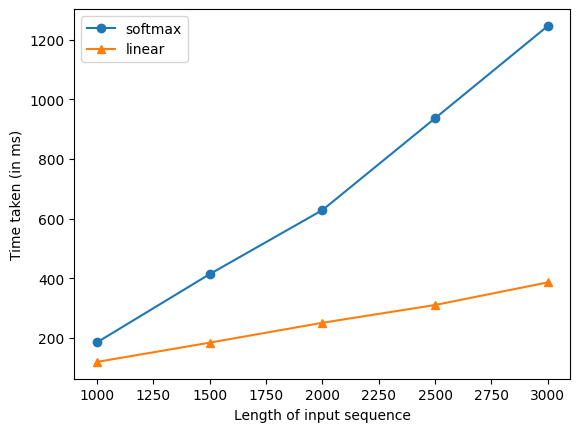
\includegraphics[width=0.4\textwidth]{images/attentiontimemeasure.png}&
             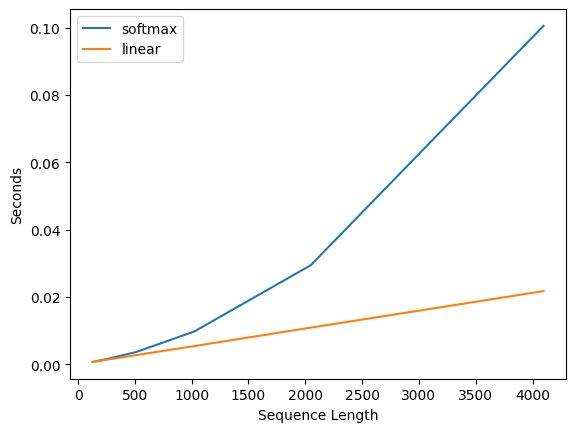
\includegraphics[width=0.4\textwidth]{images/forbacvstime.png}\\
             Time taken by attention layer & Time taken for one pass \\
            \end{tabular}  
        \end{center}
    \end{frame}

    \begin{frame}{Image Completion}
        \begin{tabular}{cccccc}
             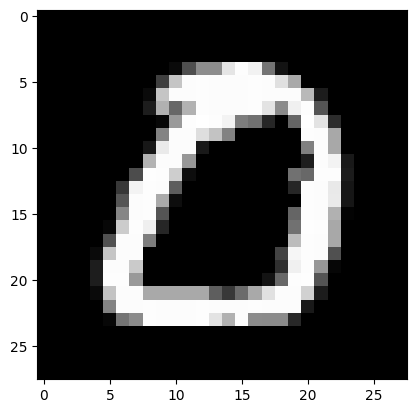
\includegraphics[width=0.1\textwidth]{images/0.png} & 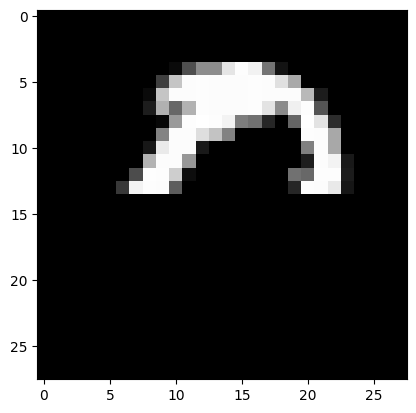
\includegraphics[width=0.1\textwidth]{images/0.5.png} & 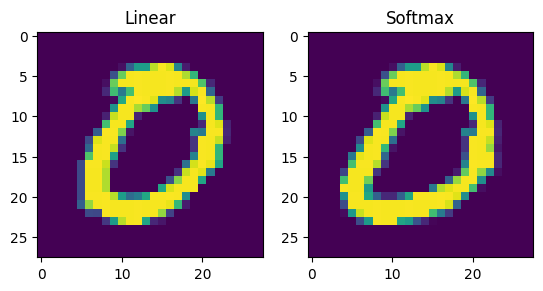
\includegraphics[width=0.2\textwidth]{images/pred0.png} & 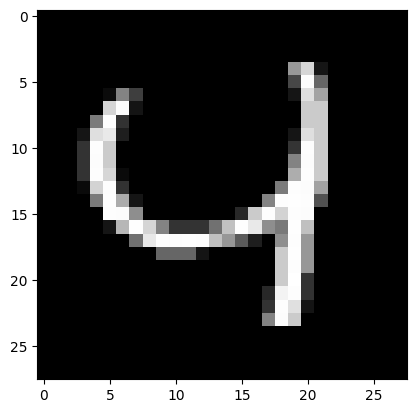
\includegraphics[width=0.1\textwidth]{images/4.png} & 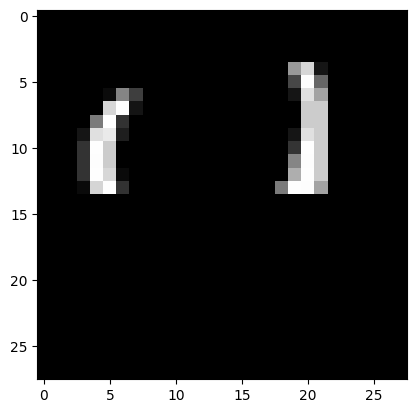
\includegraphics[width=0.1\textwidth]{images/4.5.png} & 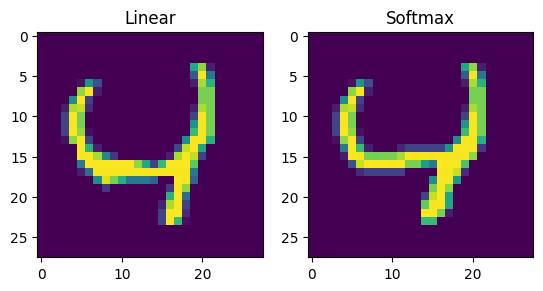
\includegraphics[width=0.2\textwidth]{images/pred4.png}\\
             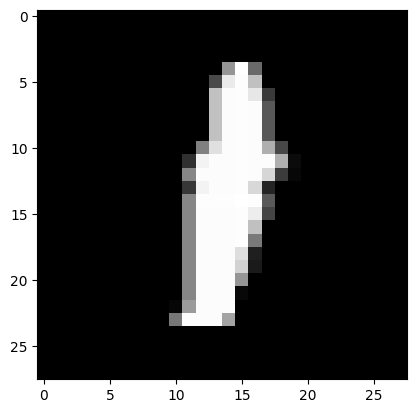
\includegraphics[width=0.1\textwidth]{images/1.png} & 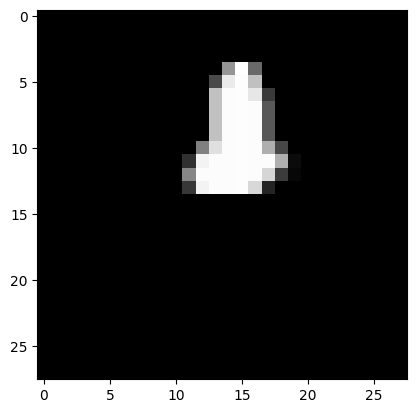
\includegraphics[width=0.1\textwidth]{images/1.5.png} & 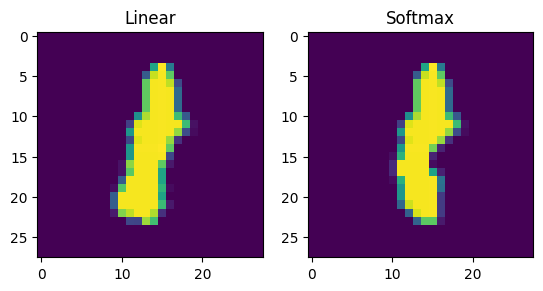
\includegraphics[width=0.2\textwidth]{images/pred1.png} & 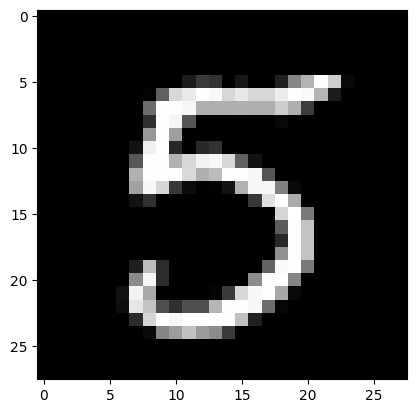
\includegraphics[width=0.1\textwidth]{images/5.png} & 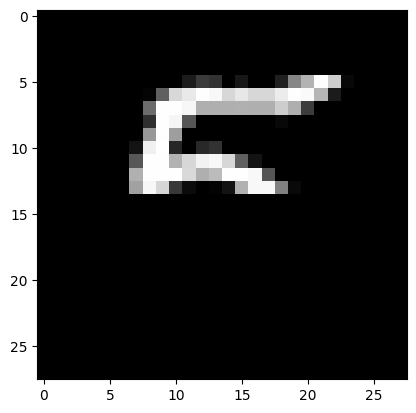
\includegraphics[width=0.1\textwidth]{images/5.5.png} & 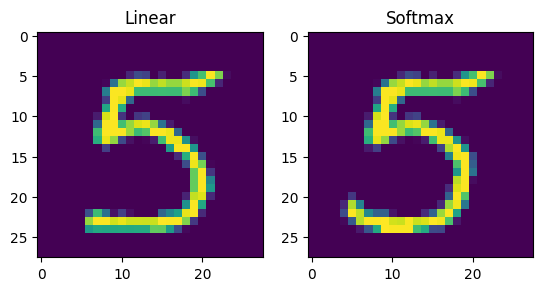
\includegraphics[width=0.2\textwidth]{images/pred5.png}\\
             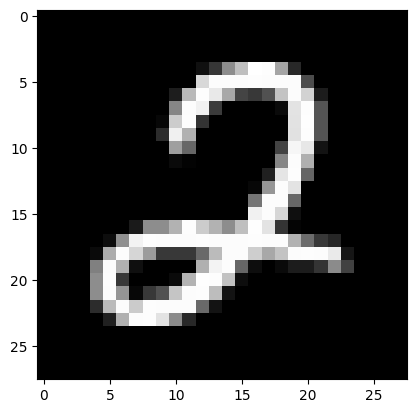
\includegraphics[width=0.1\textwidth]{images/2.png} & 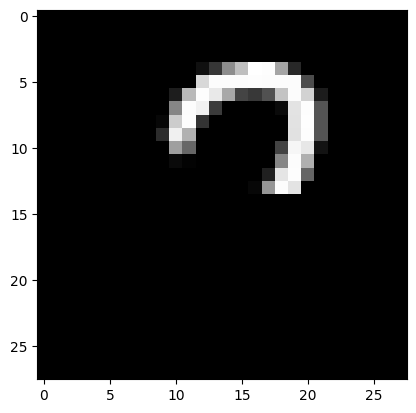
\includegraphics[width=0.1\textwidth]{images/2.5.png} & 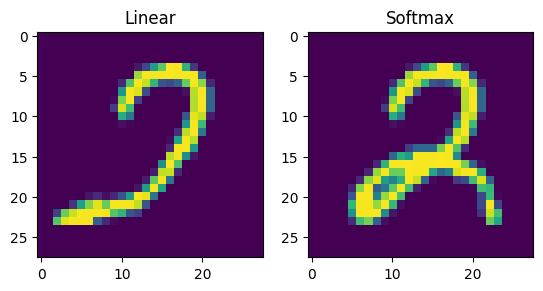
\includegraphics[width=0.2\textwidth]{images/pred2.png} &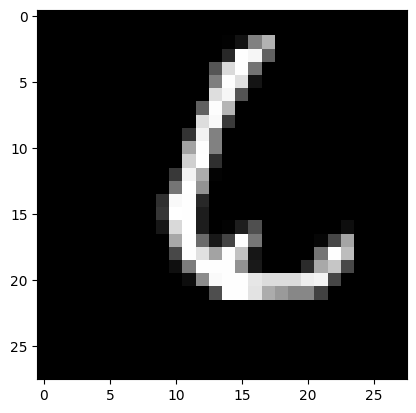
\includegraphics[width=0.1\textwidth]{images/6.png} & 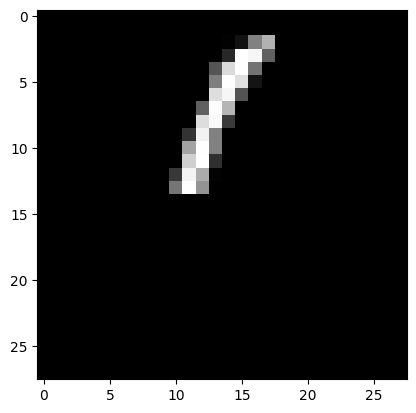
\includegraphics[width=0.1\textwidth]{images/6.5.png} & 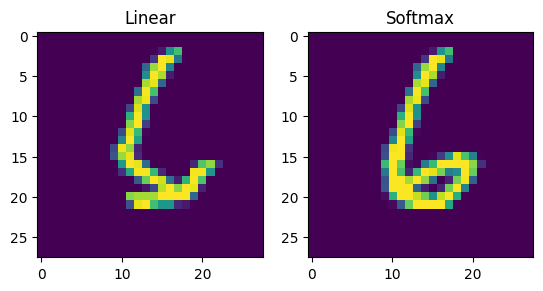
\includegraphics[width=0.2\textwidth]{images/pred6.png} \\
             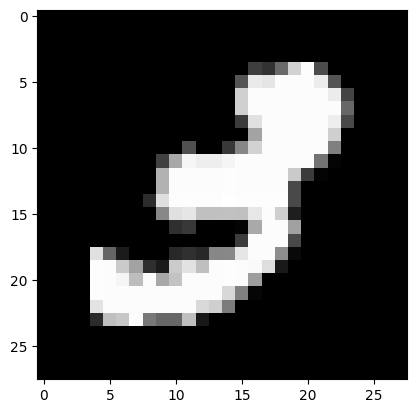
\includegraphics[width=0.1\textwidth]{images/3.png} & 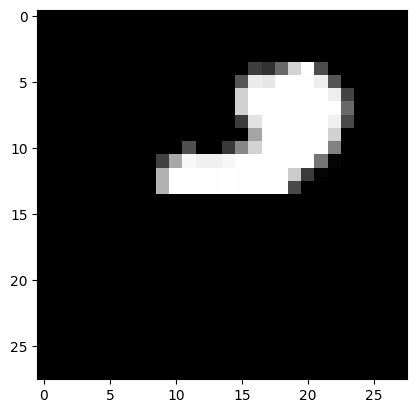
\includegraphics[width=0.1\textwidth]{images/3.5.png} & 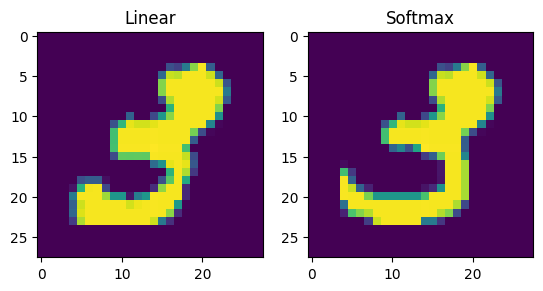
\includegraphics[width=0.2\textwidth]{images/pred3.png} & 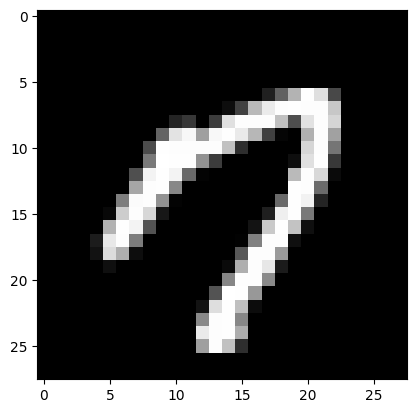
\includegraphics[width=0.1\textwidth]{images/7.png} & 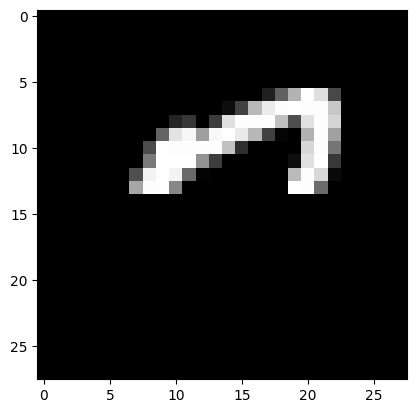
\includegraphics[width=0.1\textwidth]{images/7.5.png} & 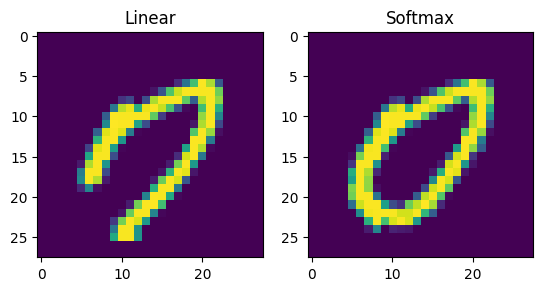
\includegraphics[width=0.2\textwidth]{images/pred7.png}
        \end{tabular}
    \end{frame}
    
    \begin{frame}{Image Completion}
        The {\color{red}linear transformer} achieved {\color{red}faster image completion} on occluded inputs in comparison to the {\color{red}softmax transformer}.
        
        
        The {\color{red}accuracies} were {\color{red}87\% and 86.3\%} on images generated by the linear and the softmax transformers respectively.
    \end{frame}
    
    \begin{frame}{Image Generation}
        \begin{table}[]
            \centering
            \begin{tabular}{|c|c|c|}
                \hline
                 Number of images& Linear & Softmax \\ \hline
                 100 & 33.45s & 367.91s \\ \hline
                 200 & 67.76s & 811.99s \\ \hline
                 300 & 76.46s & 1248.12 \\ \hline
            \end{tabular}
            \caption{Time taken for image completion}
        \end{table}

        \begin{enumerate}
            \item Quadratic nature of self-attention is clearly visible in the plots shown above.
            \item As expected, linear self-attention is way faster than softmax self-attention.
        \end{enumerate}
    \end{frame}
    
    
    \begin{frame}
    \frametitle{LoRA}
    % \framesubtitle{Mrigank}
    LoRA uses a simple property that,
     a matrix $M \in \mathbb{R}^{n \times m}$ can be rank decomposed as $M = UV$ where $U \in \mathbb{R}^{n \times r}$, $V \in \mathbb{R}^{r \times m}$ and $r$ is the rank of $M$. This reduces the number of trainable parameters from $mn$ to $r(n + m)$. Note that $r(n + m) \ll nm$ for small $r$.
    \end{frame}
    
    \begin{frame}
        \frametitle{Application of LoRA on Neural Networks}
        We have trained a feed forward neural network for an image classification task using the MNIST dataset. Our base model was composed of three linear layers which together had 55.1K trainable parameters.
        % Our objectives are as follows:
        % \begin{enumerate}
        %     \item Evaluate the robustness of the trained model on variants of the MNIST dataset without any fine-tuning.
        %     \item Fine-tune the model on the variants of the MNIST dataset and assess its performance.
        %     \item Apply LoRA during the fine-tuning of the model on the variants of the MNIST dataset and examine its performance.
        %     \item Train the neural network from scratch using LoRA and evaluate the resulting accuracies.
        % \end{enumerate}
    \end{frame}

        \begin{frame}
        \frametitle{Image Variations}
        We create variations of the MNIST dataset to finetune and test the robustness of the model.

        \begin{center}
            \begin{tabular}{@{}cccc@{}}
                
\includegraphics[width=0.15\textwidth]{images/normal_5.png} &
                
\includegraphics[width=0.15\textwidth]{images/quantized_5.png} &
                
\includegraphics[width=0.15\textwidth]{images/rotated_5.png} &
                
\includegraphics[width=0.15\textwidth]{images/inverted_5.png} \\
                MNIST & Quantized MNIST & Rotated MNIST & Inverted MNIST
            \end{tabular}
        \end{center}
    
    \end{frame}
    \begin{frame}
        \frametitle{LoRA on Neural Networks}
        \framesubtitle{Base Model Performance on Various Datasets}
    
        After training, our base model achieved a test accuracy of approximately 93.2\% on the original MNIST dataset. The performance of the model on modified datasets is presented in the table below.
    
        \begin{table}[h]
        \centering
        \begin{tabular}{|c|c|}
        \hline
        Dataset & Accuracy \\
        \hline
        Original MNIST & 93.2\% \\
        Quantized MNIST & 85.58\% \\
        Rotated MNIST & 12.38\% \\
        Inverted MNIST & 5.52\% \\
        \hline
        \end{tabular}
        \end{table}
    \end{frame}
    \begin{frame}
        \frametitle{LoRA on Neural Networks}
        \framesubtitle{Fine-tuning the model on the variants of the MNIST dataset}
        We fine-tuned our base model on three variants. 
        \begin{table}[h]
        \centering
        \begin{tabular}{|c|c|c|c|}
        \hline
        Dataset Accuracy & Accuracy & Trainable Parameters \\
        \hline
        Quantized MNIST  &  93.57\% & 55.1K \\
        Rotated MNIST & 91.97\% & 55.1K \\
        Inverted MNIST & 76.41\% & 55.1K \\
        \hline
        \end{tabular}
        \end{table}
    \end{frame}
        \begin{frame}
        \frametitle{LoRA on Neural Networks}
        \framesubtitle{Applying LoRA during fine-tuning}
        We found that our fine-tuned models achieved accuracies comparable to their full fine-tuned counterparts with fewer trainable parameters.
        \begin{center}
            \small % This line reduces the font size
            \setlength{\tabcolsep}{5pt} % This line reduces the column spacing
            \begin{tabular}{c | c | c | c | c}
                $r$ & Trainable Params & Quant. MNIST & Rot. MNIST & Inv. MNIST \\
                \hline
                1 & 1.1K & 91.20\% & 37.53\% & 16.23\% \\
                2 & 2.1K & 91.30\% & 49.01\% & 17.92\% \\
                4 & 4.2K & 91.42\% & 69.10\% & 16.32\% \\
                8 & 8.4K & 91.39\% & 77.49\% & 32.19\% \\
                16 & 16.8K & 91.72\% & 86.95\% & 62.26\% \\
                32 & 33.6K & 92.31\% & 89.50\% & 68.06\% \\
                64 & 67.2K & 93.19\% & 90.41\% & 71.88\%
            \end{tabular}
        \end{center}        
    \end{frame}
        \begin{frame}
        \frametitle{LoRA on Neural Networks}
        \framesubtitle{Applying LoRA during fine-tuning}
        \begin{center}
            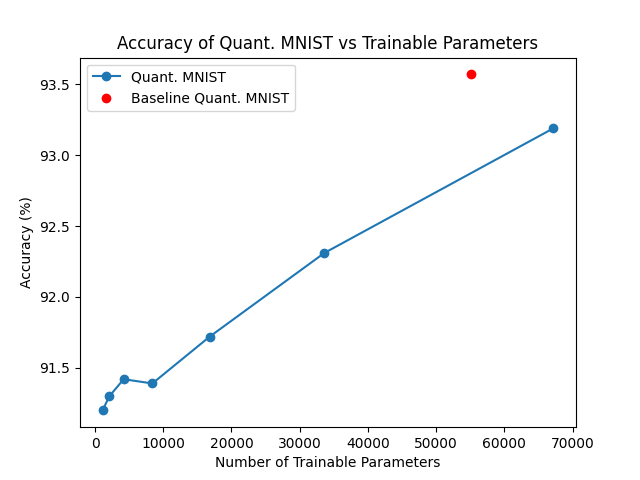
\includegraphics[width=0.8\textwidth]{images/Quantised fine tune plot.png} % Adjust the width as needed
        \end{center}
    \end{frame}
    
    \begin{frame}
        \frametitle{LoRA on Neural Networks}
        \framesubtitle{Applying LoRA during fine-tuning}
        \begin{center}
            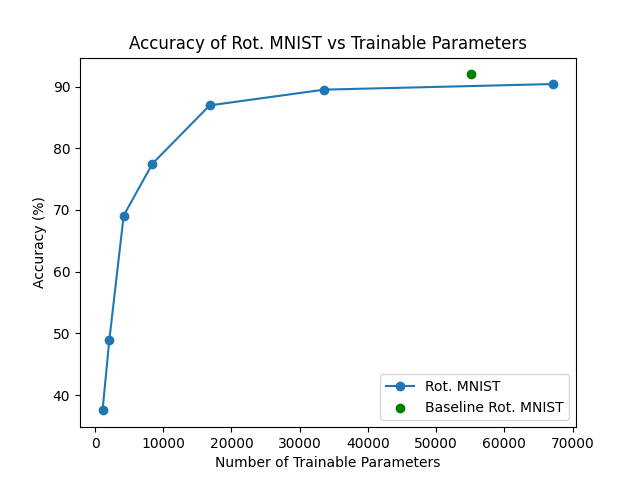
\includegraphics[width=0.8\textwidth]{images/rot mnist plot.png} % Adjust the width as needed
        \end{center}
    \end{frame}
    
    \begin{frame}
        \frametitle{LoRA on Neural Networks}
        \framesubtitle{Applying LoRA during fine-tuning}
        \begin{center}
            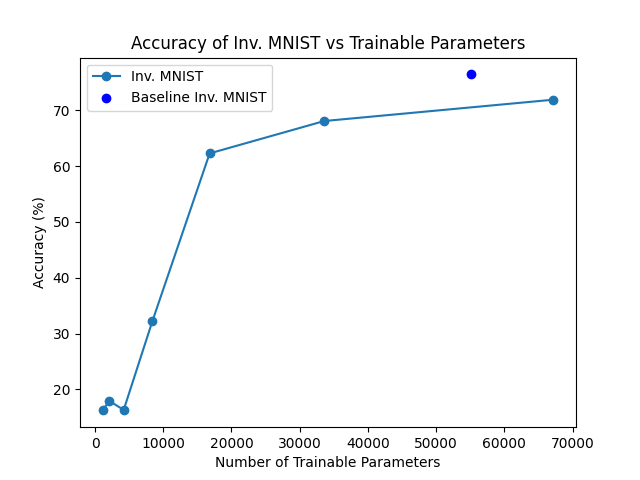
\includegraphics[width=0.8\textwidth]{images/inverse mnist plot.png} % Adjust the width as needed
        \end{center}
    \end{frame}
    \begin{frame}
        \frametitle{LoRA on Neural Networks}
        \framesubtitle{Training with LoRA from scratch}
        We trained the model from scratch with LoRA applied to the 3 layers in our neural network. The accuracy  of the models are presented in the table below.
        \begin{center}
            \small % This line reduces the font size
            \setlength{\tabcolsep}{1pt} % This line reduces the column spacing
            \renewcommand{\arraystretch}{1.2} % Adjusts the row height
            \begin{tabular}{c | c | c | c | c | c}
                \hspace{0.1cm}$r$\hspace{0.1cm} & \hspace{0.1cm}Trainable Params\hspace{0.1cm} & \hspace{0.1cm}MNIST\hspace{0.1cm} & \hspace{0.1cm}Quant. MNIST\hspace{0.1cm} & \hspace{0.1cm}Rot. MNIST\hspace{0.1cm} & \hspace{0.1cm}Inv. MNIST \\
                \hline
                1 & 1.1K & 56.79\% & 23.50\% & 25.91\% & 22.21\% \Tstrut \\
                2 & 2.1K & 71.90\% & 37.48\% & 43.96\% & 45.81\% \\
                4 & 4.2K & 84.44\% & 64.87\% & 62.60\% & 69.67\% \\
                8 & 8.4K & 89.12\% & 77.96\% & 82.39\% & 83.11\% \\
                16 & 16.8K & 92.64\% & 88.2\% & 86.76\% & 87.38\% \\
                32 & 33.6K & 93.98\% & 90.13\% & 90.62\% & 90.25\% \\
                64 & 67.2K & 94.85\% & 91.66\% & 91.85\% & 86.01\%
            \end{tabular}
        \end{center}               
    \end{frame}

    \begin{frame}
        \centering Thank You For Your Attention!
    \end{frame}
    
    \begin{frame}
      \frametitle{References}
      \nocite{*}
      \printbibliography
      \vspace{10cm}
    \end{frame}
    
    % \begin{frame}
    % \frametitle{References}
    
    % % \nocite{*} % Include all entries from the BibTeX file
    
    % % \bibliographystyle{plain} % Choose your bibliography style
    % \end{frame}

\end{document}
